\documentclass{article}
\usepackage{johd}
\usepackage[english]{babel}
\usepackage[utf8]{inputenc}

% Importing Graphics
\usepackage{graphicx}

\usepackage{listings}

% Colors for code
\usepackage{xcolor}
\definecolor{codegreen}{rgb}{0,0.6,0}
\definecolor{codegray}{rgb}{0.5,0.5,0.5}
\definecolor{codepurple}{rgb}{0.58,0,0.82}
\definecolor{backcolour}{rgb}{0.95,0.95,0.92}

\lstdefinestyle{mystyle}{
	commentstyle=\color{codegreen},
	keywordstyle=\color{magenta},
	numberstyle=\tiny\color{codegray},
	stringstyle=\color{codepurple},
	basicstyle=\ttfamily\footnotesize,
	breakatwhitespace=false,         
	breaklines=true,                 
	captionpos=b,                    
	keepspaces=true,                 
	numbers=left,                    
	numbersep=5pt,                  
	showspaces=false,                
	showstringspaces=false,
	showtabs=false,                  
	tabsize=2
}

\lstset{style=mystyle}


\title{CSE 4020 Machine Learning \\ Lab Assessment - 1  }
\author{Sujay Kumar M 20BDS0294\\ \small Computer Science Engineering with Specialization with DataScience\\ \tt sujaykumarreddy.m2020@vitstudent.ac.in
\\ \url{https://github.com/sujaykumarmag/CSE4020}}



\begin{document}
\maketitle
\section{Making a DataSet}
I made a Student Dataset with 10 Columns and 22 rows \\\\\\\
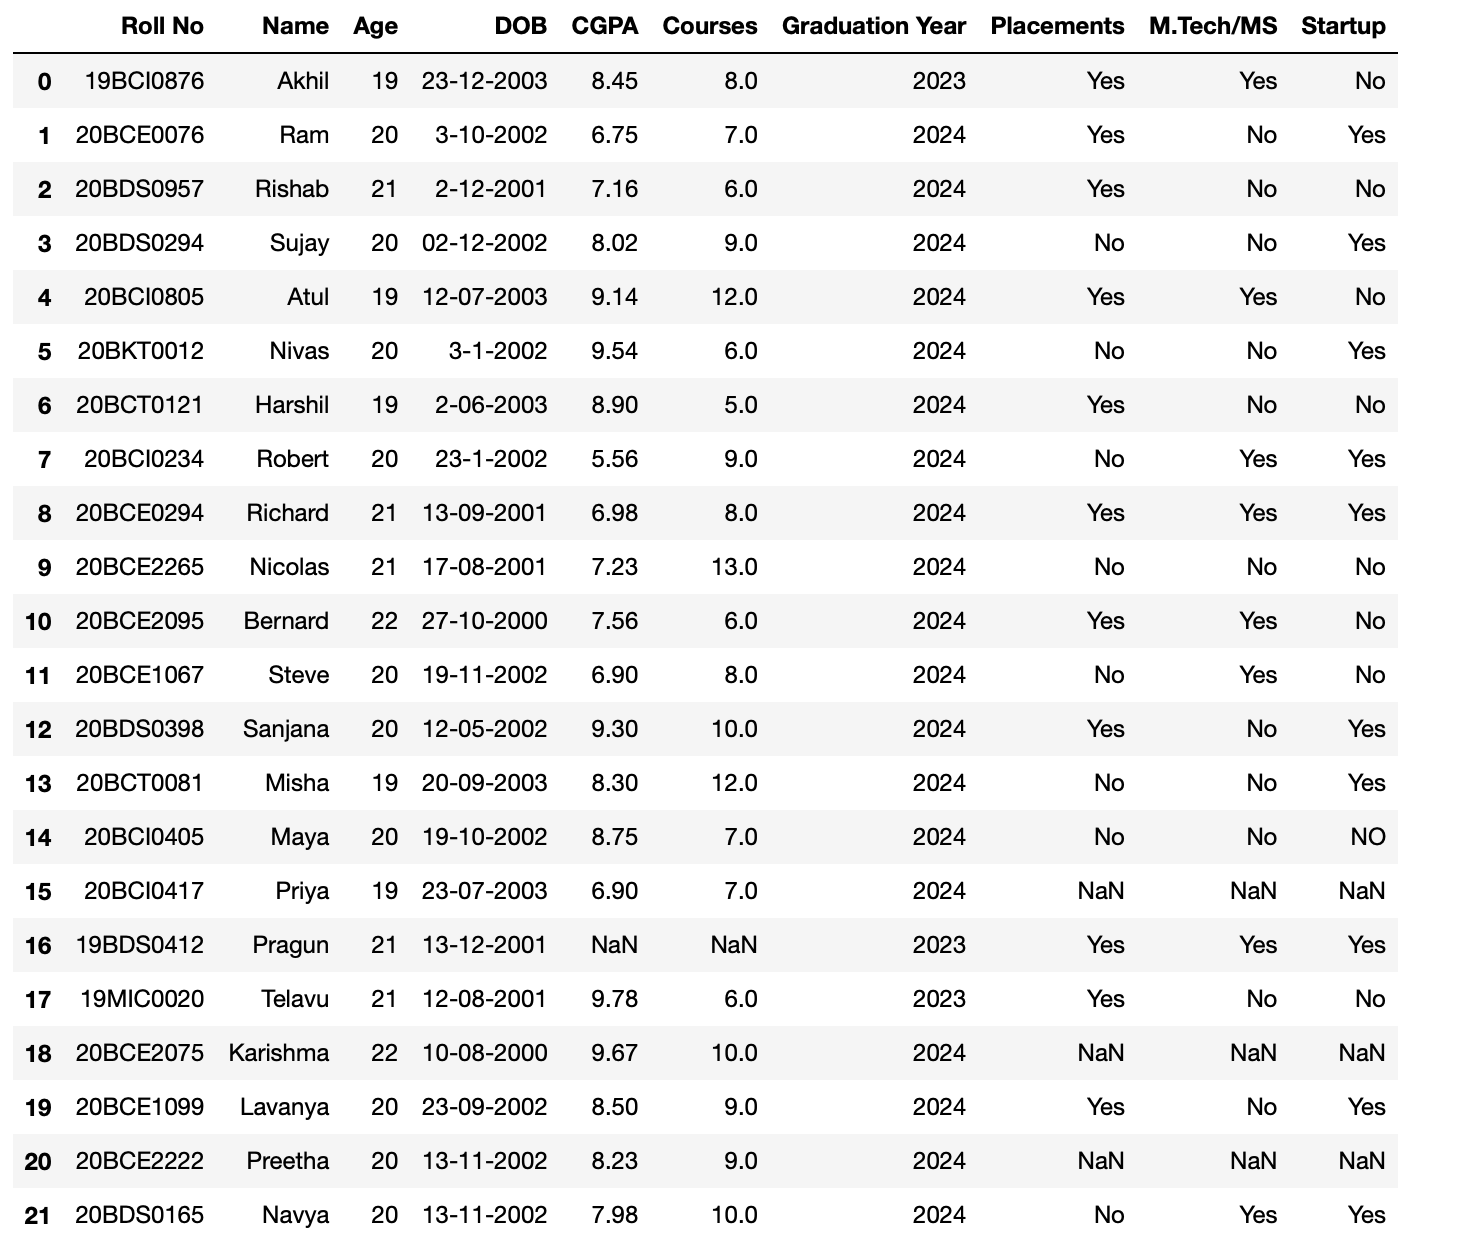
\includegraphics[scale=0.63]{images/one.png}

\section{Data Manipulation Techniques}
\subsection{Insertion}
\begin{lstlisting}[language=Python]
# Insert a column
data.insert(10,"Govt Exams","Yes")

# Insert a Row
df={
    "Roll No":["20BCE0049"],
    "Name":["Samridh"],
    "Age" :[20],
    "DOB":["10-12-2002"],
    "CGPA":[9.95],
    "Courses":[10],
    "Graduation Year":[2024],
    "Placements":["Yes"],
    "M.Tech/MS":["Yes"],
    "Startup":["No"],
    "Govt Exams":["Yes"]
}
new_row = pd.DataFrame(df)
new_row.to_csv('Untiled.csv', mode='a', index=False, header=False)
data = data.append(new_row)

# Insert a Cell
data.iloc[0,1]="Sahil"

\end{lstlisting}

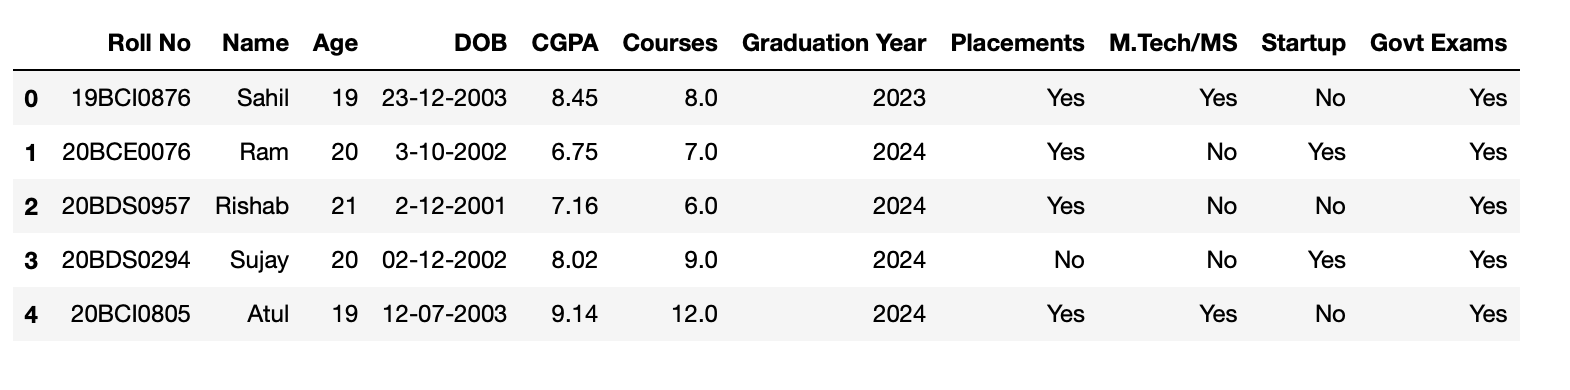
\includegraphics[scale=0.65]{images/two.png}
\subsection{Delection}
\begin{lstlisting}[language=Python]
# Delete a Column
data = data.drop("Govt Exams",axis=1)

# Delete a Row
data = data.drop(0,axis=0)

# Delete a Cell
data.iloc[1,2]="NaN"
    
\end{lstlisting}
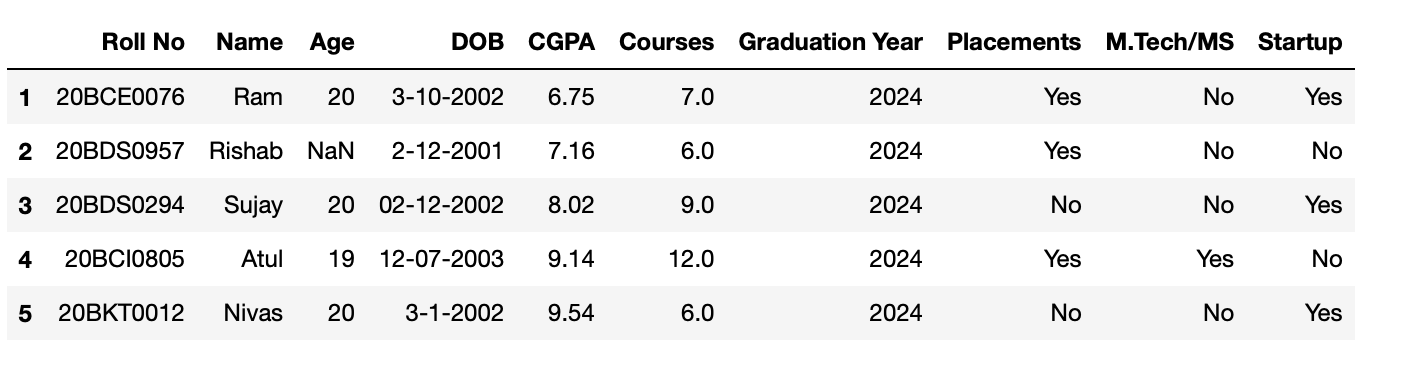
\includegraphics[scale=0.65]{images/three.png}\\\\\
\subsection{Updation}
I wanted-ly left out most of the attributes to be NaN because to impute data by using Mean, Median Mode
\begin{lstlisting}[language=Python]
# Update a Column
# arr = ["Yes","No","Yes","No","Yes","Yes","No","Yes","Yes","No","Yes","Yes","No","Yes","Yes","No","Yes","Yes","No","Yes","Yes","No","Yes","Yes"]
data[["Govt Exams"]]="No"

# Update a Row
data.iloc[0]=pd.DataFrame=({
    "Roll No":"19BCI0876",
    "Name":"Sahil Khan"
})

# Update a Cell
data.iloc[0,2]=20
    
\end{lstlisting}\\\\\\
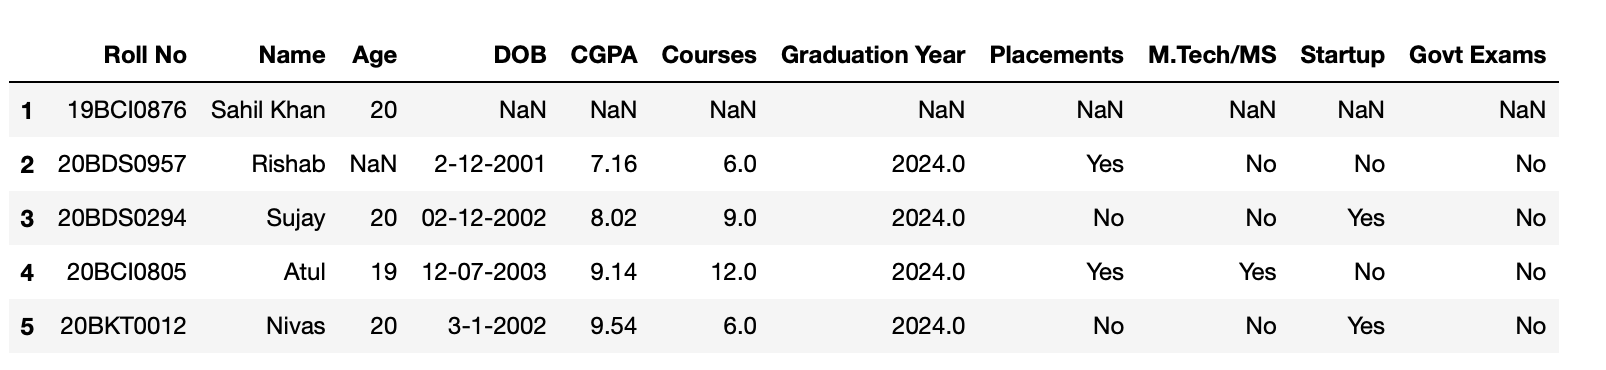
\includegraphics[scale=0.65]{images/four.png}
\section{Data Pre-Processing}
\subsection{Statistical Techniques}
\begin{lstlisting}[language=Python]
data.dtypes

data.var()

data.isnull().sum()
    
\end{lstlisting}\\\\\
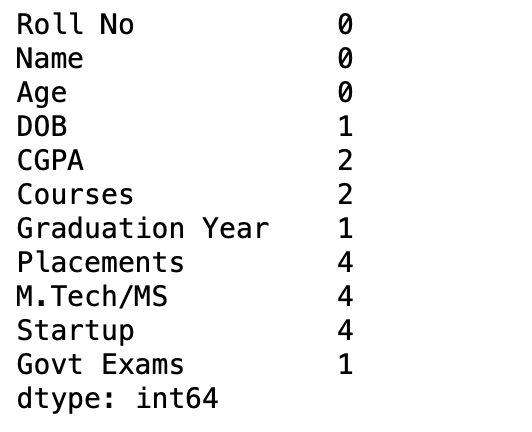
\includegraphics[sclae=0.5]{images/five.png}\\\\\\\

\subsection{Replace missing values by mean, median, and mode operations.}
\begin{lstlisting}[language=Python]
from sklearn.impute import SimpleImputer
imputer_mode = SimpleImputer(missing_values=np.nan,strategy='most_frequent');
imputer_mean = SimpleImputer(missing_values=np.nan,strategy='mean');
imputer_median = SimpleImputer(missing_values=np.nan,strategy='median');

# FOR MODE
mode_apply = data[["DOB","Placements","M.Tech/MS","Startup","Govt Exams"]]
imputer_mode.fit(mode_apply)
data[["DOB","Placements","M.Tech/MS","Startup","Govt Exams"]] = imputer_mode.transform(mode_apply)

# FOR MEDIAN
median_apply = data[["CGPA","Courses"]]
imputer_median.fit(median_apply)
data[["CGPA","Courses"]] = imputer_median.transform(median_apply)

# FOR MEAN
mean_apply = data[["Graduation Year"]]
imputer_mean.fit(mean_apply)
data[["Graduation Year"]] = imputer_mean.transform(mean_apply)
    
\end{lstlisting}\\\\\
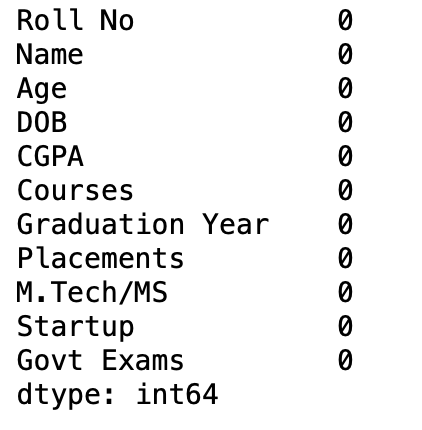
\includegraphics[scale=0.90]{images/six.png}

\subsection{Encoding Techniques}
\begin{lstlisting}[language=Python]
# ORDINAL TO CATEGORICAL
# One-hot Encoding (As there's no perfect way to do ione-hot encoding in this dataset)
from sklearn.preprocessing import OneHotEncoder
enc = OneHotEncoder(handle_unknown='ignore')
# enc.fit(X)
data.shape


# BINARY ENCODING
data["Placements"] = data["Placements"].apply(lambda row : 1 if row=='Yes' else 0)
data["Govt Exams"] = data["Govt Exams"].apply(lambda row : 1 if row=='Yes' else 0)
data["Startup"] = data["Startup"].apply(lambda row : 1 if row=='Yes' else 0)
data["M.Tech/MS"]= data["M.Tech/MS"].apply(lambda row : 1 if row == 'Yes' else 0)

# TEXT TO NUMERIC
data["Graduation Year"] = data["Graduation Year"].apply(pd.to_numeric)
data["Placements"] = data["Placements"].apply(pd.to_numeric)
data["Startup"] = data["Startup"].apply(pd.to_numeric)
data["M.Tech/MS"] = data["M.Tech/MS"].apply(pd.to_numeric)
data["Govt Exams"] = data["Govt Exams"].apply(pd.to_numeric)
data["Courses"] = data["Courses"].apply(pd.to_numeric)
data["Age"] = data["Age"].apply(pd.to_numeric)


\end{lstlisting}\\\\\\
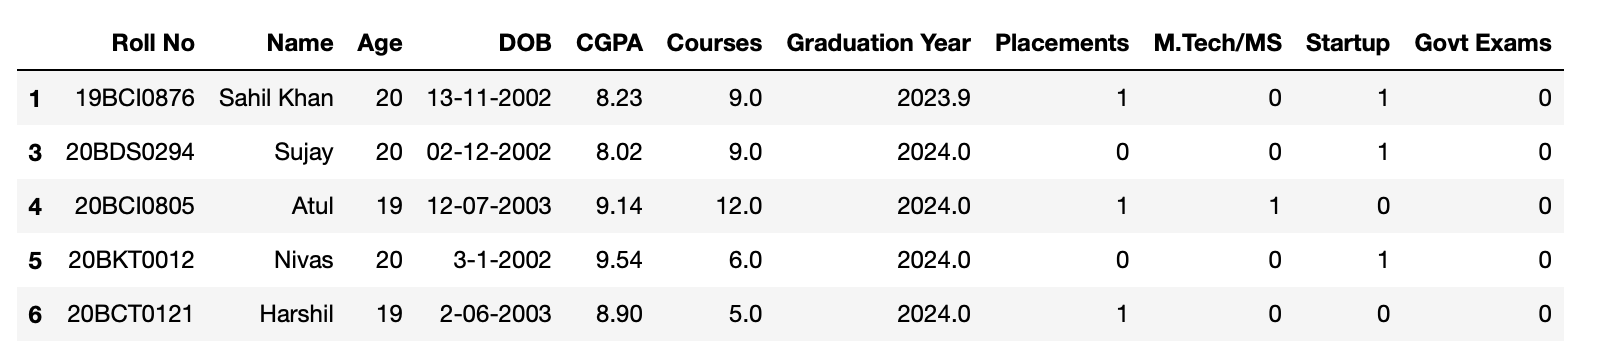
\includegraphics[scale=0.55]{images/seven.png}

\section{Normalization Techniques}
\begin{lstlisting}[language=Python]
# TRAIN-TEST SPLIT
X = data.drop(["Roll No","Name","DOB",'M.Tech/MS','Startup', 'Govt Exams'],axis=1)
y = data[["CGPA"]]
from sklearn.model_selection import train_test_split
X_train, X_test, y_train, y_test = train_test_split(X,y , test_size=0.33, random_state=42)

# MIN-MAX SCALAR
from sklearn.preprocessing import MinMaxScaler
norm = MinMaxScaler().fit(X_train)
X_train_norm = norm.transform(X_train)
X_test_norm = norm.transform(X_test)

# STANDARD SCALAR
from sklearn.preprocessing import StandardScaler
sc_X = StandardScaler()
sc_X = sc_X.fit_transform(X_train)

    
\end{lstlisting}\\\\\
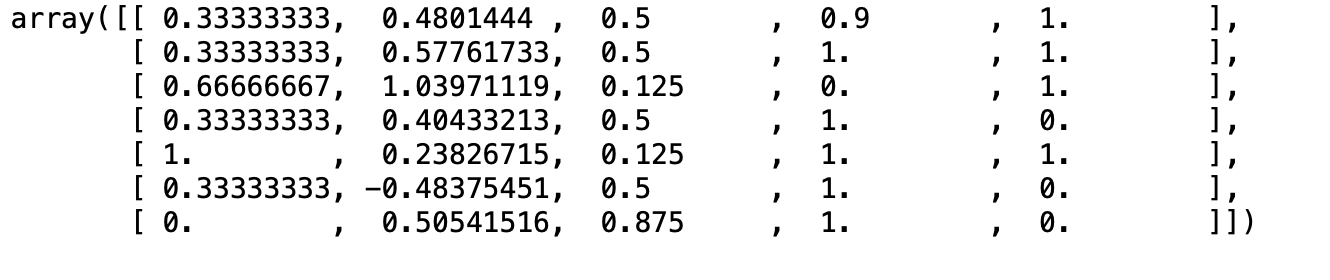
\includegraphics[scale=0.75]{images/nine.png}\\\\\\
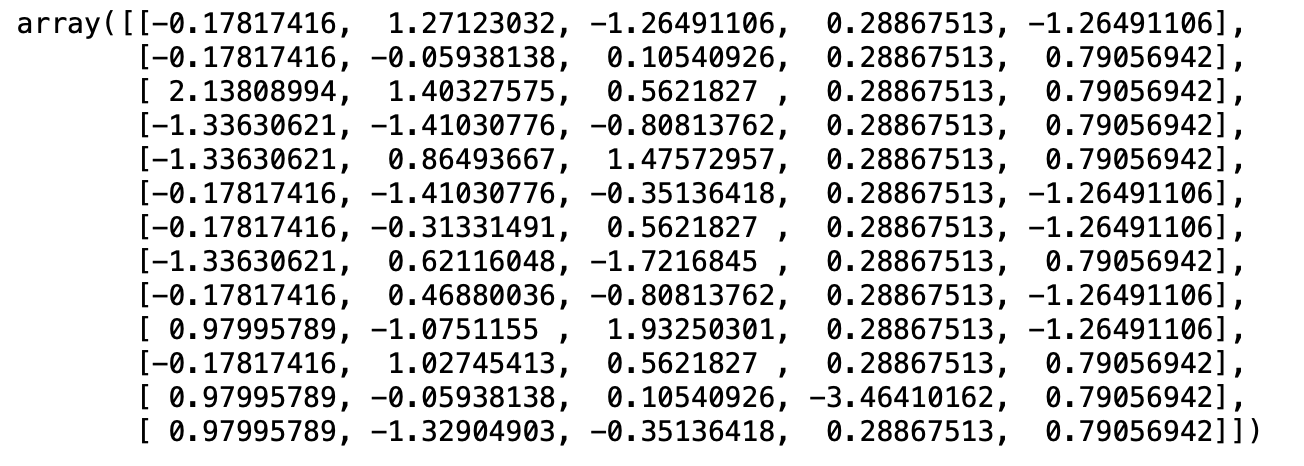
\includegraphics[scale=0.75]{images/eight.png}
\end{document}
